\chapter{绘制杯立体图}\label{chap:bei}

盛夏,太阳无情的炙烤着大地,树上的知了有气无力的鸣叫着,热浪袭卷着整个城市,人们大多都呆家中或有空调的地方以躲避酷热。秦奋前几日收到了重点高中的取通知书,兴奋过后生活又归于平淡。没有学习压力的他每天除了看电视、上网之外便无事可做。没过几日,好学地他便寻思着找到点来什么事来做或者学点什么。正琢磨着,秦奋的爸爸下班回家了,他灵光一闪:爸爸是高级工程师,他的AutoCAD用得很好,我为什么不跟他学学用AutoCAD绘图,一来可以消磨无聊的生活,二来也可以学项本事,何乐而不为呢!

秦奋立刻去冲了一杯热茶,来到爸爸的书房。爸爸看见儿子端着茶进来,心理很高兴,接过来轻轻地喝了一口,说道:“儿子,谢谢!这可是杯及时雨啊,爸爸的喉咙都快冒烟了!"说完正准备继续看书,见儿子没有走,便问:“儿子还有什么事吗?是不是想玩会儿电脑啊?”

秦奋很认真地说道:“爸,我也没有什么特别的事,只事想跟你学学用AutoCAD,平时学习任务重想跟你学,却没有时间。现在离开学还有一个多月的时间,也没有别的学习任务,你看能不能教教我啊?”

爸爸看看认真的秦奋,会心一笑,说:“儿子长大了,想学技术了,而且还是爸爸会的技术,你说我能不愿意教吗?”

{\bfseries 知识目标}
\begin{itemize}
\item 掌握line命令的使用
\item 掌握offset命令和trim命令的使用
\item 掌握circle命令
\item 掌握端点和圆心捕捉方法
\item 掌握AutoCAD视图切换知识
\item 掌握AutoCAD旋转和拉伸建模命令的使用方法
\item 掌握AutoCAD差集命令的使用方法
\end{itemize}

{\bfseries 技能目标}
\begin{itemize}
\item 能够根据给定的回转体零件图,运用投影知识选择正确的投影图
\item 能够根据块零件特征,运用AutoCAD命令,绘制特征图
\item 能够运用AutoCAD旋转和拉伸命令,完成回转体零件和平面体块零件的三绘建模
\end{itemize}

{\bfseries 本章提要}

本章将对调压阀中的杯零件进行三维建模,使读者能够掌握line命令、offset命令和trim命令绘制简单回转体零件特征视图的方法,并通过实体建模中revolve命令和extude命令来生成三维模型。通过完成该项目读者能够基本掌握使用AutoCAD进行三维建模的基本步骤。图\ref{fig:tiaoyafabei}所示即为本项目的块零件图。
\noindent
\begin{figure}[htbp]
\centering
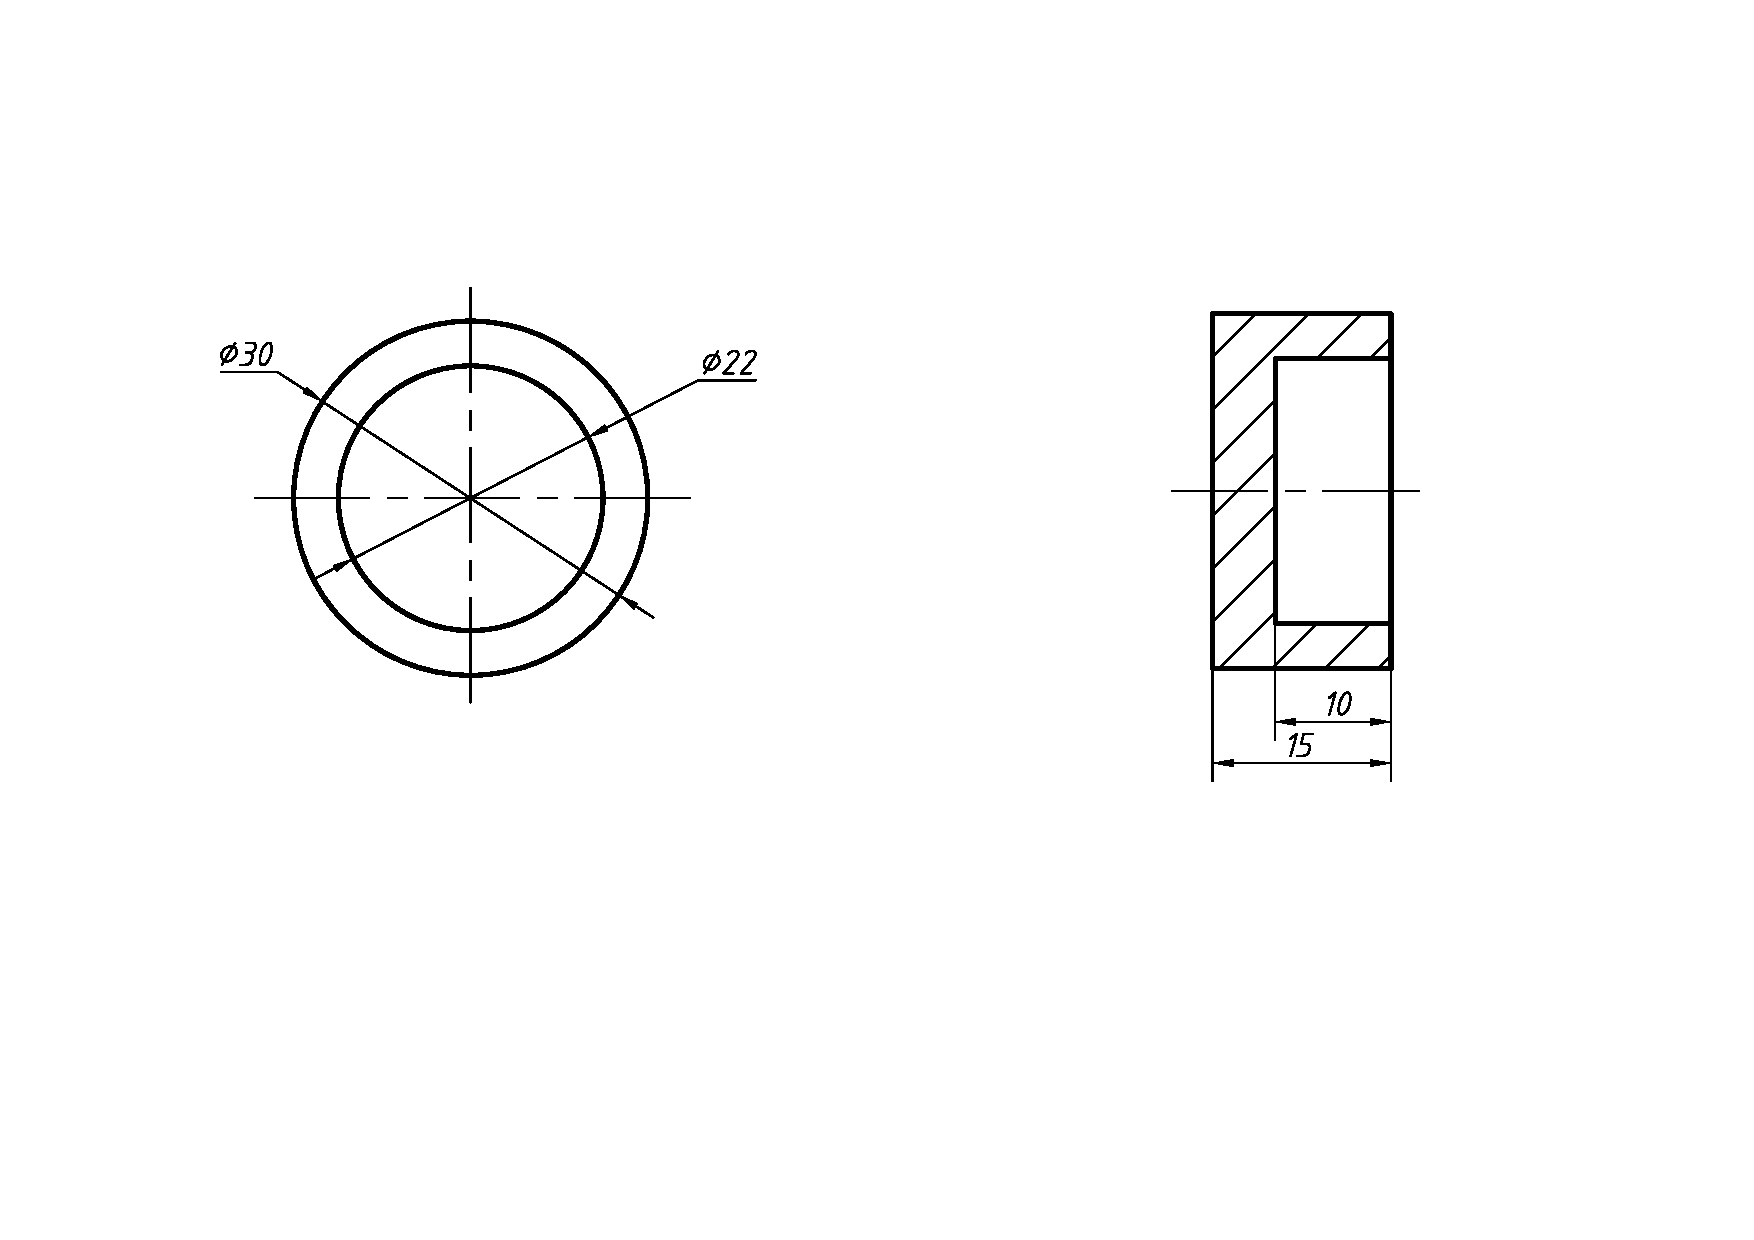
\includegraphics[scale=0.6]{tiaoyafabei.pdf}
\caption{杯零件图}\label{fig:tiaoyafabei}
\end{figure}
\endinput